\section{Materiales y Métodos}

Como parte de la metodología para llevar a a cabo el experimento se tomó como base el esquema de la figura 1, en el que se destacan tres fases del proceso de detección de patrones a partir del electroencefalograma o EEG: Pre-procesamiento de la señal, extracción y clasificación de características. El primer paso cosnsiste en  eliminar el ruido, como los artefactos o el ruido de la línea de alimentación que se agrega al EEG.

En nuestro caso, no llegaremos a la predicción del caracter, sino tan sólo nos quedaremos con la clasificación de los P300.

\begin{figure}[t]
    \centering
    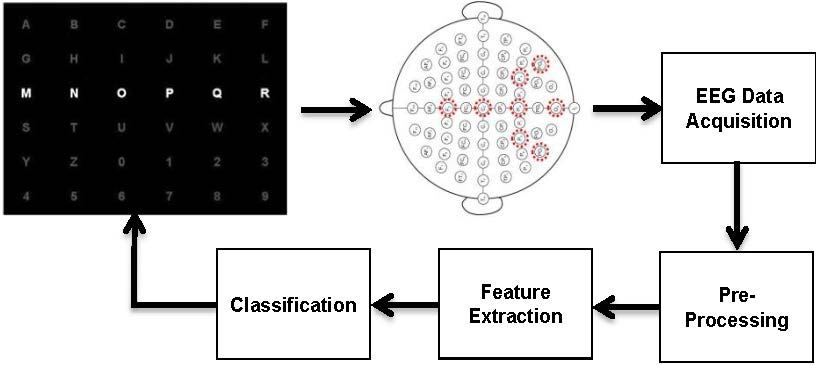
\includegraphics[width=\textwidth]{P300BCI.jpg}
    \caption{Configuración típica de un P300 BCI con relimentación visual.}
    \label{fig:P300BCI}
\end{figure}


\subsection{Dataset}

El dataset consiste en grabaciones hechas en \emph{Tecnópolis}. 135 sujetos participaron del experimento, que consistió en deletrear palabras preestablecidas para calibrar el sistema (etapa de entrenamiento), y luego un modo \emph{free-riding} en el cual los sujetos podían utilizar el speller libremente. Sólo se recopiló la parte de entrenamiento.

En cada paso, una de las filas o columnas de la matriz del speller \ref{fig:Matrix6x6} se intensifica aleatoriamente durante 100 ms. A continuación, todas las filas y columnas se desactivaron durante 75 ms. Esto continúa hasta que se enciendan 12 filas y columnas para cada carácter. 

Se utilizó un EMOTIV, un headset de bajo costo que consiste sólo de 14 electrodos, con un sampling rate de 128 hz. Se aplicó un filtro FIR de fase cero entre 0 y 20 hz. 

La señal de EEG se separó en instancias (epochs) de la siguiente manera: por cada estímulo (flash en la matriz de letras) se tuvo en cuenta los 100 ms previos (utilizados para la estabilización de la señal) y los 700 restantes al estímulo. Es decir, si el estímulo ocurrió en tiempo $t$, se obtuvo la instancia $(t-100, t+700)$. Esto nos da 104 muestras por los 14 canales.

Para el tratamiento de los archivos resultantes, se utilizó la librería de Python \emph{MNE} \cite{gramfort2014mne}.


\subsection{Normalización}

Para mejorar la performance del clasificador, trasladamos y re-escalamos los datos de la siguiente manera:

\begin{equation*}
    I_{i, j} = (I_{i, j} - \bar{I_i}) / \sigma_i
\end{equation*}
    
donde $I(i, j)$ representa el voltaje medido en el electrón $i$ en tiempo $j$, $ \bar{I_i})$ y $\sigma_i$ representan el valor medio y la desviación estándar del electrón $i$. Estas normalizaciones se efectuaron por sujeto. 


\subsection{Topología de la Red}

La red consta de dos capas convolucionales, seguidas de una capa densa y finalmente de una salida que indica la probabilidad de que la entrada se corresponda con un potencial P300. 

De manera similar a lo que suele hacerse en el área de BCI, nuestra red efectúa: en primer lugar se buscan combinaciones óptimas de canales, para luego efectuar una extracción de características en base a patrones (por ejemplo, Fourier y Wavelets). En ese sentido, la estructura de la red es bastante comprensible.

Las capas convolucionales que implementan dichos filtrados (primero en espacio y luego en tiempo) son o bien vectores columna o fila, para evitar que el filtrado se centre en electrodos que no tienen continuidad espacial. 

Así, la topología de la red es la siguiente:

\begin{itemize}
    \item $L_0$: Capa de entrada, $I_{i,j}$ con tamaño $14 \times 104$.
    \item $L_1$: Capa convolucional, con 12 filtros de tamaño $(14, 1)$. \item $L_2$: Capa convolucional, con 60 filtros de tamaño $(1, 13)$.
    \item $L_3$: Capa densa, totalmente conexa a la capa anterior.
    \item $L_4$: Capa de salida, consta de una neurona.
\end{itemize}

Las funciones de activación utilizadas son \emph{reLU} para todas las capas, salvo para la salida que utiliza una función de activación sigmoidea.

Esta topología (a la que denominaremos $CNN-1$) fue la básica. Probamos otras combinaciones:

\begin{itemize}
    \item $CNN-2$: Agregamos una capa de \emph{max-pooling} inmediatamente después de la segunda capa convolucional.
    \item $CNN-3$: Dos capas convolucionales seguidas de \emph{max-pooling}
\end{itemize}

\subsubsection{Entrenamiento y regularización}

La red se entrenó utilizando el algoritmo \emph{rmsprop}\cite{tieleman2012lecture} con \emph{entropía cruzada} como función de pérdida. Para evitar el overfitting, utilizamos en conjunto dos técnicas:

\begin{itemize}
    \item Early Stopping: Se separó un pequeño subconjunto de validación para ir verificando que por cada \emph{epoch} (en el sentido de Redes Neuronales) la función de pérdida tenga una mejora. Si no es así luego de 3 epochs, se detiene el entrenamiento
    \item Dropout: con cierta probabilidad $p$, se ponen, en un paso del entrenamiento, a 0 las entradas de una capa. Esto evita que las unidades se ``co-adapten'' demasiado.
\end{itemize}

Se utilizó la librería de Python \emph{keras}\cite{chollet2015} para su implementación.
